\chapter{Overview of \textsf{\mdseries {Flycatcher}}}
The development of Flycatcher can be divided into distinct phases, which correspond to the components of the application. In order for the reader to follow and understand the development process, we feel that it is best to start off by giving them a sense of the big picture. Hence, in this chapter we will explain our choice of programming environment, briefly describe the stages involved and give an overview of the system.

\section{Environment}
\subsection{V8 engine}

In picking a JavaScript engine to work with to develop \textsf{Flycatcher}, we looked for the following characteristics:
\begin{itemize}
   \item developer friendliness
   \item a standalone release (many are coupled with browsers)
   \item speed of execution
   \item open source
   \item strong online community
   \item conform to the latest ECMAScript standard, ECMA-262 edition 5
   \item meta-programming features
   \item runs on x86 or x86-64 processors
\end{itemize}

Of the three main contenders in these categories, namely Firefox's SpiderMonkey and Rhino engines and Google's V8, V8 was chosen as it was by far the strongest, notably in terms of execution speed and developer friendliness. The version of V8 used is 3.9.5.

\subsection{Node.js framework}
\begin{figure}[h]
%\hspace*{0.2cm}
\centering

\includegraphics[scale=0.2]{./components/chapter3/nodejs.png}
\end{figure}

JavaScript's debut on the server side prompted the need for a form of application development library support for the language. The development of \emph{Node.js} that started in 2009 was an attempt to satisfy this need. Although the framework is intended as an event-driven web framework, the fact that it has a strong online developer community and a variety of valuable open source contributions makes it appealing for developing JavaScript in general. It is all the more appealing to us because it is built on top of the V8 JavaScript engine, which is our engine of choice.

On top of its built-in library support, Node.js offers an efficient package manager \texttt{npm}, which allows us to effectively separate our work into components, as well as easily import plugins from the open source community. The Node.js release used to deveop \textsf{Flycatcher} is version 0.7.5.


\section{Design}
The process of automatically generating tests using the approach we have chosen, dynamic test generation, naturally divides into distinct stages. In this section we will outline and briefly describe what those stages are and introduce the components of the application that they correspond to.

\subsection{Components}
\subsubsection{Analysing the source}
The very first task that \textsf{Flycatcher} needs to perform is a dynamic \emph{analysis} of the source code, in order to extract information about the program under test. The \textsf{Analyser} component performs this role: extracting the information that is necessary to even start the test generation process at all. Intuitively, we can think of it as mapping the source code into \textsf{Flycatcher}'s data structures, which are then used in the test generation process.

\subsubsection{Generating candidate tests}
% TODO GENETIC The next component involved is the \textbf{Test Generator}, which has two implementations consisting of a random test generator to start off with followed by a search-based generator for improved efficiency. 
The following stage consists in generating \emph{candidate} or \emph{eligible} tests. These generated tests are run inside a custom runtime environment and depending on the \emph{feedback} provided by that environment, they may be eligible to become part of the final suite of unit tests which is output to the user. The early tests are not accurately typed and therefore not eligible, but serve to gather runtime information until we have enough information to generate tests that are. As such, the \textsf{Test Generator} component which fulfils this role is tightly coupled with another: the one which orchestrates a virtual runtime environment in order to collect the necessary runtime information.

\subsubsection{Developing a custom runtime environment}
The custom runtime environment which is necessary to run candidate tests and provide feedback on their eligibility, is implemented by the \textsf{Executor} component. Its main responsibilities are:
\begin{enumerate}
   \item enabling the collection of information concerning the type of method parameters
   \item tracking the code coverage achieved by candidate tests, to assess their quality
\end{enumerate}

The \textsf{Executor} and the \textsf{Test Generator} thus work in to-and-fro until either full code coverage is achieved or a termination criterion is met. Upon termination, the tests that are deemed accurately typed and that contributed to code coverage are collated into a suite of unit tests. They are then output to the user in a format corresponding to his preferred unit testing framework. The tests that reveal an error in the program under test or a possible mistake made by \textsf{Flycatcher}'s type inference mechanism are also output, as \emph{failing tests}.

\subsection{System}
Figure \ref{system} gives an idea of the overall system and how the components fit together, so that the reader can appreciate the journey from the program under test to a suite of test cases that can be used for regression unit-testing.

\begin{figure}[h]
\centering
% \hspace*{-0.3cm}
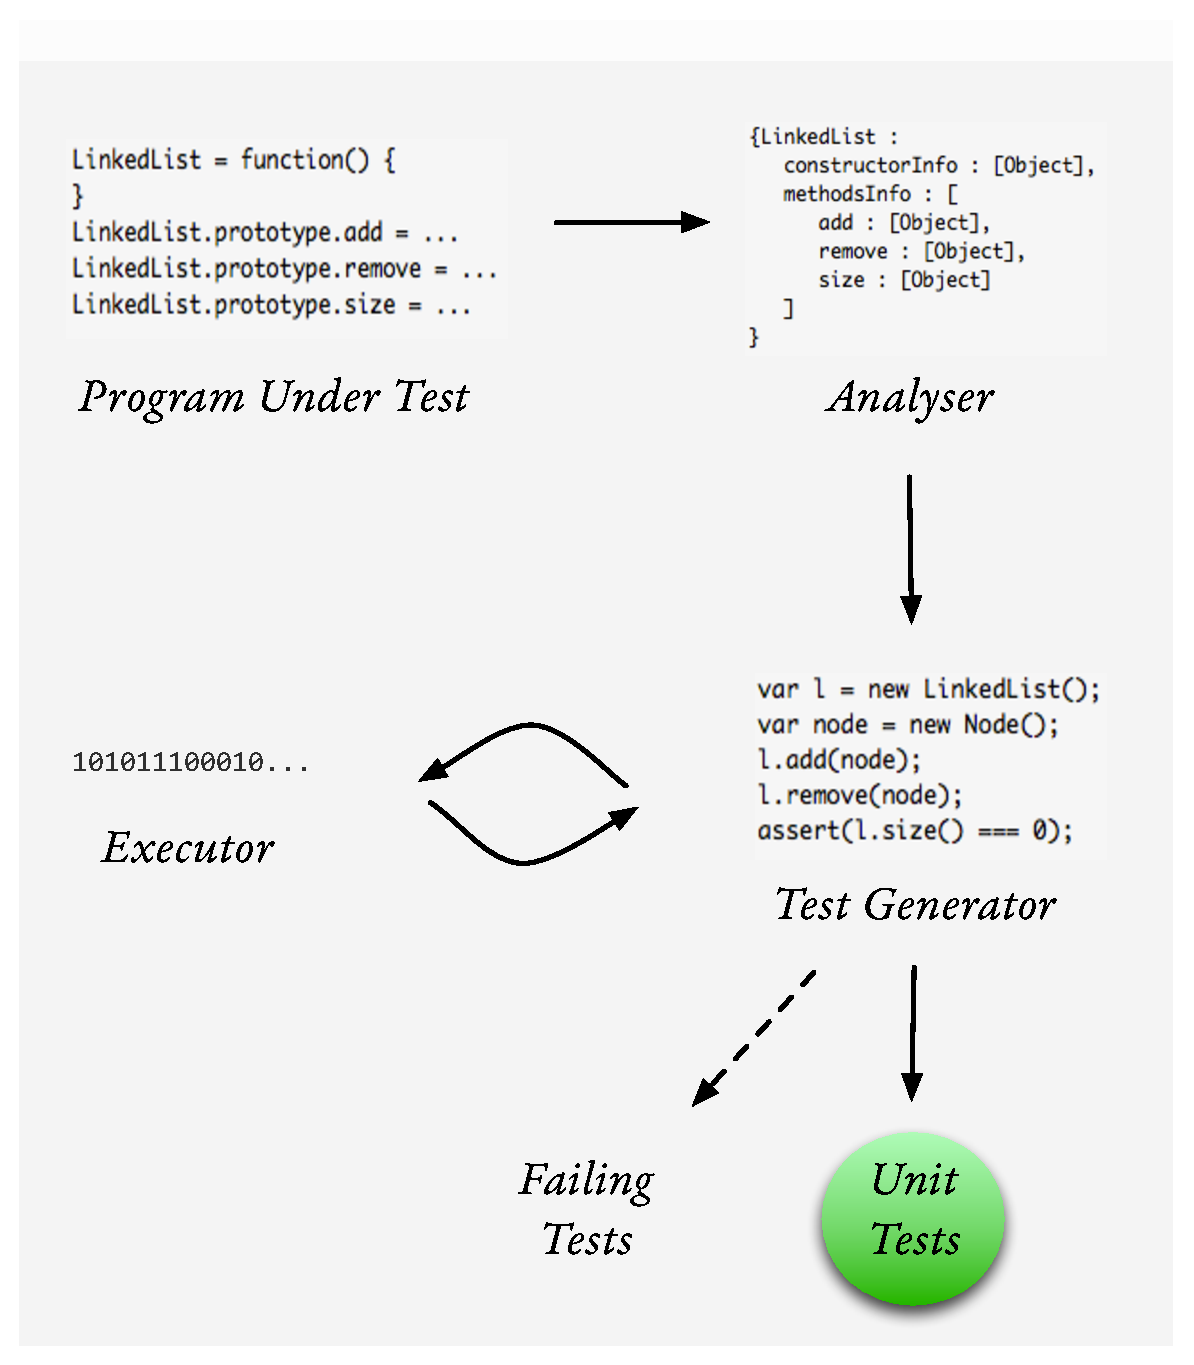
\includegraphics[scale=0.55]{./components/chapter3/system9.pdf}
\caption{The \textsf{Flycatcher} system}
\label{system}
\end{figure}

\section{JavaScript support}
In this section, we elaborate on which JavaScript features are supported by \textsf{Flycatcher}. First of all, there are two separate matters to consider:

\begin{enumerate}
   \item the support for JavaScript inside the classes being tested
   \item the support for JavaScript concerning the types of parameters
\end{enumerate}

Given that \textsf{Flycatcher} is built on one of the latest versions of the V8 engine, it supports all of the ECMAScript Edition 5 constructs \emph{inside} the classes under test.

However, there are limitations when it comes to the support for the \emph{parameters}' types, due to the fact that these types will need to be inferred by \textsf{Flycatcher}, and there are restrictions as to what types \emph{can} be. Flycatcher supports the inference of the primitive types \emph{number}, \emph{string} and \emph{boolean} and therefore also their object counterparts \texttt{Number}, \texttt{String} and \texttt{Boolean}. Additionally, \textsf{Flycatcher} supports used-defined types, as long as their definition is accessible in the source code under test. However, it is worth noting that there is currently no support for other standard objects, including \texttt{Array} and \texttt{Function}, due to the technical challenge they represent. Finally, there is no support for the parameters to be literal objects \emph{i.e.} objects must belong to a class, which is in line with the object-oriented style targeted by this tool. This is also appropriate in the context of unit tests, as they are meant to test the external interface of a self-contained unit. The elements of that interface must therefore be of a well-known primitive or user-defined type. Nevertheless, the lack of support for \texttt{Array} and \texttt{Function} does have its drawbacks, which we will discuss in the evaluation chapter.

\section{\textsf{\mdseries{Flycatcher}} usage}
\label{usagesection}
\begin{figure}[h]
\hspace*{-2cm}
\centering
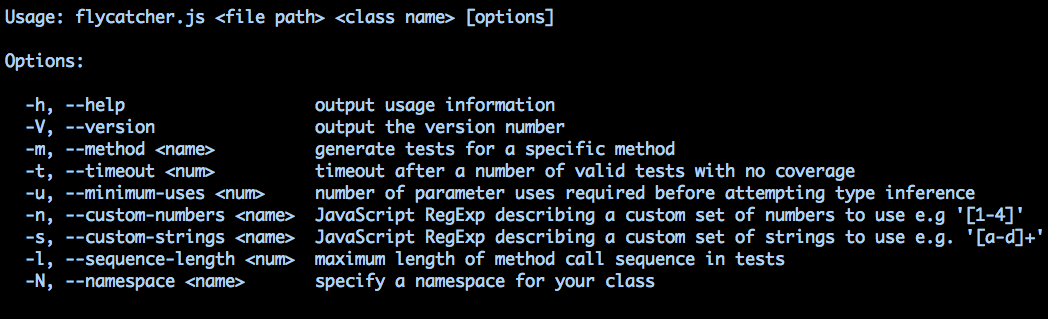
\includegraphics[scale=0.45]{./components/chapter7/params.png}
\caption{\textsf{Flycatcher} parameters}
\label{usage}
\end{figure}

\textsf{Flycatcher}'s usage information can be seen in the screenshot in Figure \ref{usage}. The required arguments are the source file where the class under test can be found as well as the name of that class. The following arguments are optional:

\begin{itemize}
   \item \texttt{\textendash \textendash method <name>}: Specifying a single method from the class under test, tests are only generated for that method. If this is not specified, tests are generated for all of the class under test's methods.
   \item \texttt{\textendash \textendash namespace <name>}: This option serves to specify a namespace inside which to look for the class under test in case it is not available in the global context.
   \item \texttt{\textendash \textendash out <name>}: Specifying a file for the tests to be output. The unit-test suite is output in \texttt{<name>.js} and the failing tests are output in \texttt{<name>.log}. If this is not specified the tests are output in a default file.
   \item \texttt{\textendash \textendash custom-strings and \textendash \textendash custom-numbers <re>}: So that the random input strings and numbers that are generated by \textsf{Flycatcher} for the unit tests are \emph{appropriate} for the program under test, custom generators can be specified for each. These are specified by a string \texttt{<re>} which represents a regular expression that conforms to the JavaScript RegExp syntax. For example, to generate only strings between \emph{a} and \emph{f}, one would use \texttt{"[a-f]+"}.
   \item \texttt{\textendash \textendash timeout <num>}: Indicates termination after \texttt{<num>} \emph{valid}\footnote{tests for which we have already inferred types for all parameters involved} tests are generated without achieving any coverage. This number indicates that the part of the code that remains to be covered is either unreachable or deeply nested. However, in the event that it is the former, a certain termination criterion is decided upon.
   \item \texttt{\textendash \textendash strict-timeout <num>}: The \texttt{\textendash \textendash timeout <num>} adapts to the program under test \emph{i.e.} if it is a program that performs long calculations this is taken into account. However, if a precise deadline is needed, it can be specified with the \texttt{strict-timeout} option.
   \item \texttt{\textendash \textendash sequence-length <num>}: Method sequences in tests are generated by \textsf{Flycatcher} at random, but in order for tests to have a reasonable size, the sequences must have a maximum length. This maximum can be specified with this option, which defaults to ten if none is specified (based on experimentation).
   \item \texttt{\textendash \textendash minimum-uses <num>}: Before types are inferred for parameters inside candidate tests, a number of tests are run inside \textsf{Flycatcher} for the sole purpose of collecting information on those parameters. Every time such a temporary test is run, we keep track of the parameters that are used for all of the functions involved. This gives us a measure of how much information has potentially been collected for each parameter \emph{i.e.} how confident a type estimate we will be able to make for that parameter at any point in time. This advanced option sets the number of parameter uses after which we consider having enough information for type inference. It defaults to twenty if not specified (based on experimentation).
\end{itemize}

% In order to understand the parameters used in the experiments carried out in this section, we give a summary of the parameters available to \textsf{Flycatcher} users. Those options can be seen in the screenshot of \textsf{Flycatcher}'s usage information in Figure \ref{params}. We then consider the parameters that can impact our experiments' results, and specify what value they will take.

% \subsection{Specifying the MUT}
% Since the collection of information about parameter types happens early on in the test generation process, when testing a whole class, methods tested later benefit from the information collected for the earlier methods. As a result, the time necessary to achieve desired coverage will be much shorter for the later methods, when the test generation process happens for an entire class, as does by default. So that we can carry out effective comparisons and evaluation, we therefore test specific methods of our benchmark classes, such that the type inference stage is taken into account every time.

% \subsection{Choosing a timeout}
% \textsf{Flycatcher}'s timeout mechanism does not consist of a fixed deadline but a more telling measure, which adapts to the program under test: the number of \emph{valid}\footnote{tests for which we have already inferred types for all parameters involved} tests that are generated without achieving any coverage. This number indicates that the part of the code that remains to be covered is either unreachable or deeply nested. However, in the event that it is the former, a certain termination criterion needs to be decided upon. For both experiments carried out in this section, the timeout chosen was \emph{5000 tests}.
% 
% \subsection{Parameter use before inference}
% A key feature of \textsf{Flycatcher} is the ability to let the user decide with how much confidence the type of parameters should be inferred. The measure of confidence in inferring a type for a parameter lies in the number of times that parameter has been used in a test. The more the parameter has been used, the more data will have been collected about its type and the stronger the type inference. \underline{The first experiment will consist in varying this parameter} to observe its effect. In the second experiment we will fix it to \texttt{10}.
% 
% \subsection{Custom data generators}
% So that the random input strings and numbers that are generated by \textsf{Flycatcher} for the unit tests are \emph{appropriate} for the program under test, custom generators can be specified for each. They are specified by a string which represents a regular expression that conforms to the JavaScript RegExp syntax. When the benchmark tests require custom data generators, these will be specified when we discuss the experiments themselves.
% 
% \subsection{Setting the maximum length for tests}
% When generating object-oriented tests, once the object under test has been initialised, a certain number of methods are called on that object in an attempt to modify its state before calling the MUT. The idea is that this improves code coverage of the MUT. However, as the length of the method call sequence in tests varies, so does the time it takes to achieve full coverage for a MUT. Increasing the length of method call sequences initially speeds up the test generation process, but the tests become too big, the overall process slows down. In trying to find the optimal value for the length of tests for each program, \underline{the second experiment will consist in varying this parameter}.

\section{\textsf{\mdseries{Flycatcher}} example}
% In figure \ref{run}, we give an example of \textsf{Flycatcher} running with the default settings for the method \texttt{getType} of the \texttt{Triangle} class (see Appendix \ref{triangle}). The \texttt{Triangle} class is instantiated with three numbers representing its sides. It has three setter methods and a \texttt{getType} method which returns the type of the triangle (equilateral, isosceles, scalene or invalid). As the screenshot shows, all of the parameter types are correctly inferred and 100\% coverage of the method under test is achieved. Additionally, \textsf{Flycatcher} indicates that it did not find any bugs in the program \emph{i.e.} all of the valid tests that it generated were added to the unit-test suite, none of them failed. Figure \ref{testexample} shows one of the tests generated by \textsf{Flycatcher} during this run.\\

\begin{figure}[t]
% \hspace*{-0.2cm}
\centering
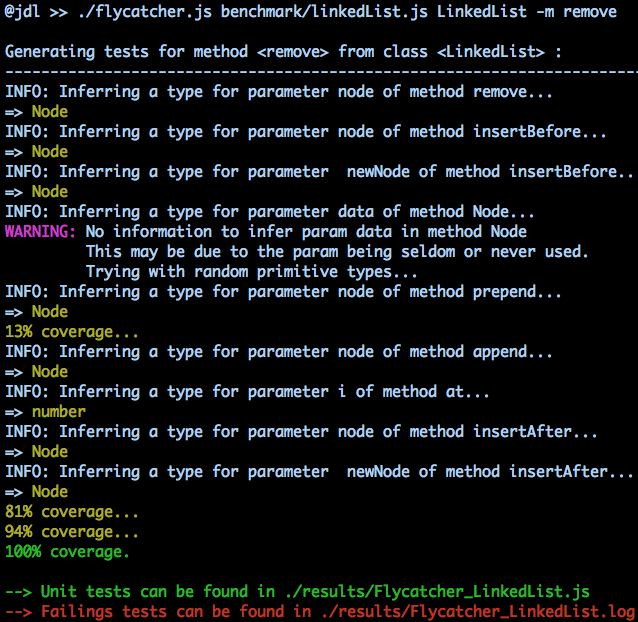
\includegraphics[scale=0.55]{./components/chapter3/lesscolour.png}
\caption{Example run}
\label{run}
\end{figure}

In figure \ref{run}, we give an example of \textsf{Flycatcher} running with the default settings for the method \texttt{remove} of the \texttt{LinkedList} class (see Appendix \ref{ll}), a standard linked list implementation. Parameters are inferred for all of the class's methods, not just the one under test, as those methods are used inside the test cases. As the command line output shows, in the early stage of the test generation process, the correct types are inferred for all the parameters when possible.

In a linked list implementation, it is often the case that the nodes' values are not used inside the implementation itself --- they are only used in the context where the linked list is used. Hence we cannot collect any information regarding the type of the \texttt{data} parameter and in order to retain as much autonomy as possible, it is substituted with a random type, here a \emph{string}. From the example we can see that 100\% test coverage is achieved for the \texttt{remove} method of the \texttt{LinkedList} class, thanks to the generated unit tests like the one in Figure \ref{testexample}. Tests that fail even though all parameter types have been resolved indicate a weakness in the program. For example, in Figure \ref{failingtest} we can see that the linked list implementation does not check when calling \texttt{insertBefore}, whether the target node exists in the list, which gives rise to a \texttt{TypeError}.\\[4cm]

\begin{code}[caption=Unit test, label=unittest]
var linkedlist325 = new LinkedList();
var node326 = new Node("AdlwkJCa2");
linkedlist325.prepend(node326);
assert.equal(linkedlist325.remove(node326), true);
linkedlist325.size();
var node327 = new Node("5asd24all");
linkedlist325.prepend(node327);
var node328 = new Node("azcma5");
assert.equal(linkedlist325.remove(node328), false);
// Success!
\end{code}

% \vspace*{0.2cm}
\begin{code}[caption=Failing test, label=failingtest]
var linkedlist309 = new LinkedList();
var node310 = new Node("J619y4xu1");
var node311 = new Node("segBPUR5");
linkedlist309.insertBefore(node310,node311);
linkedlist309.at(22);
var node312 = new Node("L93Ifj7t75");
linkedlist309.append(node312);
var node313 = new Node("9");
linkedlist309.remove(node313);
// TypeError: Cannot set property 'next' of null   
\end{code}


% \begin{figure}[b]
% % \hspace*{-0.2cm}
% \centering
% 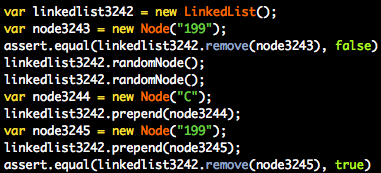
\includegraphics[scale=0.6]{./components/chapter3/linkedlisttest.png}
% \caption{Unit test}
% \label{testexample}
% \end{figure}
% 
% \begin{figure}[t]
% % \hspace*{-0.2cm}
% \centering
% 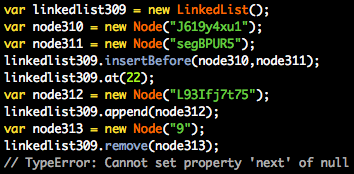
\includegraphics[scale=0.6]{./components/chapter3/linkedlistfail.png}
% \caption{Failing test}
% \label{failingtest}
% \end{figure}

% \begin{figure}[h]
% \hspace*{-2.5cm}
% \centering
% 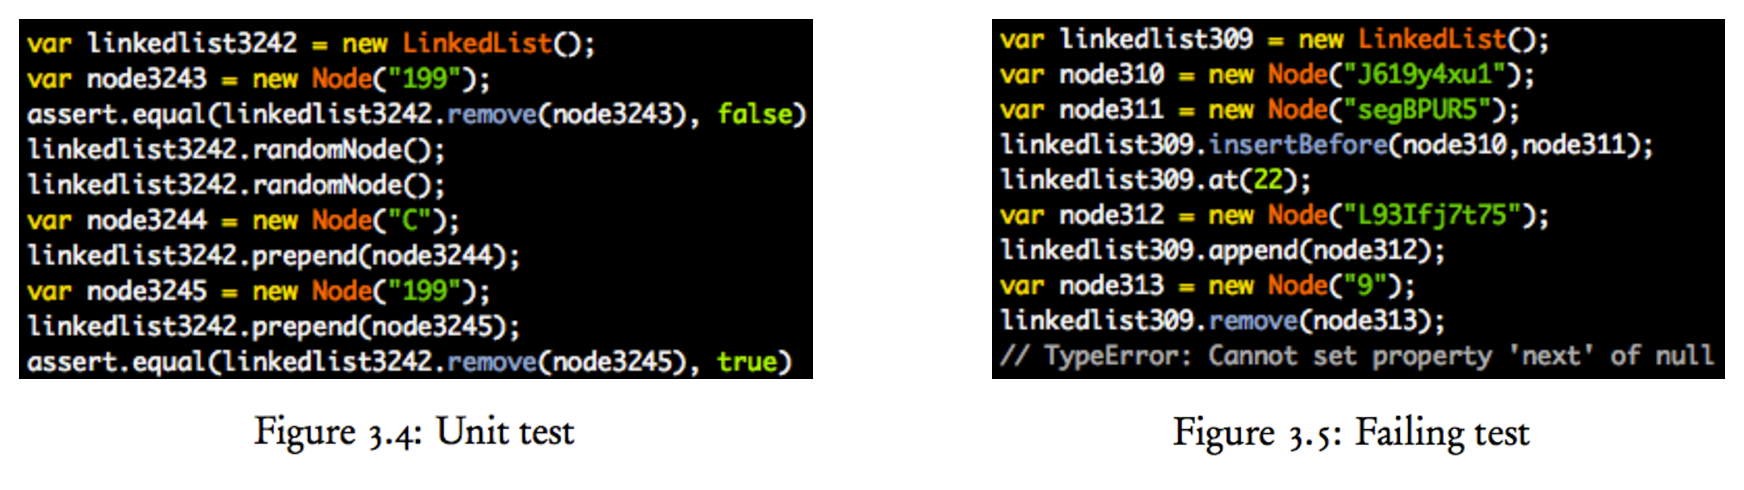
\includegraphics[scale=0.5]{./components/chapter3/linkedlistres.pdf}
% % \caption{Failing test}
% \label{testexample}
% \end{figure}
\vspace*{1cm}
In the next three chapters, we elaborate upon this high-level overview, by detailing the implementation of the three core stages described:

\begin{enumerate}
   \item Analysing the source
   \item Generating candidate tests
   \item Developing a custom runtime environment
\end{enumerate}